C++17 brought with it one major advance and several minor tweaks to concurrency-related features. Let us quickly cover the latter first. The std::lock() function that was introduced in C++11 now has a corresponding RAII object, std::scoped\_lock. A shared mutex, std::shared\_mutex, otherwise known as a read-write mutex, was added (again, matching the corresponding POSIX feature). This mutex allows multiple threads to proceed as long as they do not need exclusive access to the locked resource. Usually, such threads perform read-only operations, while a writer thread needs exclusive access, hence the name read-write lock. It's a clever idea in theory, but most implementations offer dismal performance. 

Of note is a new feature that allows portably determining the cache line size for L1 cache, std::hardware\_destructive\_interference\_size, and std::hardware\_constructive\_interference\_size. These constants help create cache-optimal data structures that avoid false sharing.

Now we come to the major new feature in C++17 – parallel algorithms. The familiar STL algorithms now have parallelized versions (overall, the set of parallel algorithms is often referred to as parallel STL). For example, here is the basic call to std::for\_each:

\begin{lstlisting}[style=styleCXX]
std::vector<double> v;
… add data to v … 
std::for_each(v.begin(), v.end(),[](double& x){ ++x; });
\end{lstlisting}

In C++17, we can ask the library to do this computation in parallel on all available processors:

\begin{lstlisting}[style=styleCXX]
std::vector<double> v;
… add data to v … 
std::for_each(std::execution::par,
			v.begin(), v.end(),[](double& x){ ++x; });
\end{lstlisting}

The parallel versions of STL algorithms have a new first argument: the execution policy. Note that the execution policy is not a single type but rather a template parameter. The standard provides several execution policies; the parallel policy std::execution::par that we used earlier allows the algorithm to execute on multiple threads. The number of threads and the way the computations are partitioned within threads are unspecified and depend on the implementation. The sequential policy std::execution::seq executes the algorithm on a single thread, the same way it's executed without any policies (or before C++17).

There is also a parallel unsequenced policy, std::execution::par\_unseq. The difference between the two parallel policies is subtle but important to understand. The standard says that the unsequenced policy allows computations to be interleaved within a single thread, which allows additional optimizations such as vectorization. But an optimizing compiler can use vector instructions like AVX when generating machine code, and it's done without any help from the source C++ code: the compiler just finds vectorization opportunities and replaces regular single-word instructions with vector ones. So what is different here?

To understand the nature of the unsequenced policies, we have to consider a more complex example. Let us say that, instead of simply operating on every element, we want to do some computation that uses shared data:

\begin{lstlisting}[style=styleCXX]
double much_computing(double x);
std::vector<double> v;
… add data to v … 
double res = 0;
std::mutex res_lock;
std::for_each(std::execution::par, v.begin(), v.end(),
[&](double& x){ 
	double term = much_computing(x);
	std::lock_guard guard(res_lock);
	res += term;
});
\end{lstlisting}

Here we do some computations on each vector element, then accumulate the sum of the results. The computations themselves can be done in parallel, but the accumulation must be protected by a lock since all threads increment the same shared variable res. The parallel execution policy is safe to use, thanks to the lock. However, we cannot use an unsequenced policy here: if the same thread were to process multiple vector elements at the same time (interleaved), it could attempt to acquire the same lock multiple times. This is a guaranteed deadlock: if a thread is holding the lock and tries to lock it again, the second attempt will block, and the thread cannot proceed to the point where it would have unlocked the lock. The standard calls code such as our last example vectorization-unsafe and states that such code should not be used with unsequenced policies. 

Now that we have seen how parallel algorithms work in theory, how about in practice? The short answer is quite well, with some caveats. Read on for the long version.

Before you can check out parallel algorithms in practice, you have to do some work to prepare your built environment. Usually, to compile C++ programs, you just need to install the desired compiler version, such as GCC, and you are ready to go. Not so with parallel algorithms. At the time this book is written, the installation process is somewhat cumbersome. 

Recent enough versions of GCC and Clang include parallel STL headers (in some installations, Clang requires GCC to be installed because it uses GCC-provided parallel STL). The problem appears at the lower level. The runtime threading system used by both compilers is Intel Threading Building Blocks (TBB), which comes as a library with its own set of headers. Neither compiler includes TBB in its installation. To complicate matters even more, each version of the compiler requires the corresponding version of TBB: neither an older nor a more recent version will work (the failures can manifest themselves at both compile and link-time). To run the programs linked with TBB, you will likely need to add the TBB libraries to your library path.

Once you have resolved all these problems and configured a working installation of the compiler and necessary libraries, using parallel algorithms is no harder than using any STL code. So, how well does it scale? We can run some benchmarks. 

Let us start with std::for\_each without any locks and with a lot of computations for each element (function work() is expensive, the exact operations don't really matter for our current focus on scaling):

\hspace*{\fill} \\ %插入空行
\noindent
\textbf{parallel\_algorithm.C}
\begin{lstlisting}[style=styleCXX]
std::vector<double> v(N);
std::for_each(std::execution::par,
v.begin(), v.end(),[](double& x){ work(x); });
\end{lstlisting}

Here is the performance of the sequential versus the parallel version running on 2 threads:

\hspace*{\fill} \\ %插入空行
\begin{center}
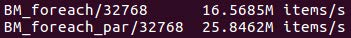
\includegraphics[width=0.9\textwidth]{content/2/chapter8/images/1.jpg}\\
Figure 8.1 – Benchmark of parallel std::foreach on 2 CPUs
\end{center}

The scaling is not bad. Note that the vector size N is fairly large, 32K elements. The scaling does improve for larger vectors. However, for relatively small amounts of data, the  performance of parallel algorithms is very poor:

\hspace*{\fill} \\ %插入空行
\begin{center}
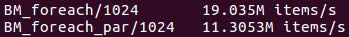
\includegraphics[width=0.9\textwidth]{content/2/chapter8/images/2.jpg}\\
Figure 8.2 – Benchmark of parallel std::foreach for short sequences
\end{center}

The parallel version is slower than the sequential version for vectors of 1024 elements. The reason is that the execution policy starts all the threads at the beginning of each parallel algorithm and joins them at the end. Launching new threads takes significant time, so when the computation is short, the overhead overwhelms any speedup we can get from parallelism. This is not a requirement imposed by the standard, but the way the current implementation of parallel STL in GCC and Clang manages its interactions with the TBB system. 

Of course, the size for which parallel algorithms improve performance depends on the hardware, the compiler and its implementation of parallelism, and the amount of computation per element. For example, we can try a very simple per-element computation:

\begin{lstlisting}[style=styleCXX]
std::for_each(std::execution::par,
v.begin(), v.end(),[](double& x){ ++x; });
\end{lstlisting}

Now processing the same 32K-element vector shows no benefit of parallelism:

\hspace*{\fill} \\ %插入空行
\begin{center}
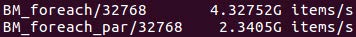
\includegraphics[width=0.9\textwidth]{content/2/chapter8/images/3.jpg}\\
Figure 8.3 – Benchmark of parallel std::foreach for cheap per-element computations
\end{center}

For much larger vector sizes, the parallel algorithm may get ahead unless memory access speed limits the performance of both single- and multi-threaded versions (this is a very much memory-bound computation). 

Perhaps more impressive is the performance of algorithms that are more difficult to parallelize, such as std::sort:

\begin{lstlisting}[style=styleCXX]
std::vector<double> v(N);
std::sort(std::execution::par, v.begin(), v.end();
\end{lstlisting}

This is the output for it:

\hspace*{\fill} \\ %插入空行
\begin{center}
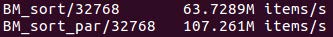
\includegraphics[width=0.9\textwidth]{content/2/chapter8/images/4.jpg}\\
Figure 8.4 – Benchmark of parallel std::sort
\end{center}

Again, we need a sufficiently large amount of data before the parallel algorithm becomes effective (for 1024 elements, single-threaded sort is faster). This is quite a remarkable achievement: sort is not the easiest algorithm to parallelize, and per-element computations on doubles (comparison and swap) are very cheap. Nonetheless, the parallel algorithm shows very good speedup, and it gets better if the element comparison is more expensive. 

You might wonder how parallel STL algorithms interact with your threads, that is, what happens if you run two parallel algorithms on two threads simultaneously? First of all, like with any code running on multiple threads, you have to ensure thread safety (running two sorts on the same container in parallel is a bad idea no matter which sort you use). Other than that, you will find that multiple parallel algorithms coexist just fine, but you have no control over job scheduling: each of them tries to run on all available CPUs, so they compete for the resources. Depending on how well each algorithm scales, you may or may not get higher overall performance by running several algorithms in parallel.

Overall, we can conclude that the parallel versions of STL algorithms deliver very good performance when they operate on large enough data volumes, although what is large enough depends on the particular computation. Additional libraries may be needed to compile and run programs that use parallel algorithms, and configuring these libraries may require some effort, as well as experimentation. Also, not all STL algorithms have their parallel equivalents (for example, std::accumulate does not).

….

We are now ready to flip a few more pages on the calendar and jump forward to C++20.














